\documentclass[10pt,a4paper]{article}
\bibliographystyle{ACM-Reference-Format}
\usepackage[colorlinks=true, urlcolor=blue, linkcolor=red]{hyperref}
\hypersetup{colorlinks=true}
\usepackage{graphicx}
\graphicspath{ {./images/} }
\usepackage{listings}
\usepackage{color}

\definecolor{dkgreen}{rgb}{0,0.6,0}
\definecolor{gray}{rgb}{0.5,0.5,0.5}
\definecolor{mauve}{rgb}{0.58,0,0.82}

\lstset{frame=tb,
	language=Python,
	showstringspaces=false,
	columns=flexible,
	basicstyle={\small\ttfamily},
	numbers=none,
	numberstyle=\tiny\color{gray},
	keywordstyle=\color{blue},
	commentstyle=\color{dkgreen},
	stringstyle=\color{mauve},
	breaklines=true,
	breakatwhitespace=true,
	tabsize=3
}

\title{}
\author{Antonio Facchiano\\Salvatore Ruocco\\Simone Vittoria}
\date{9 Gennaio 2024}

\renewcommand\contentsname{Indice}

\begin{document}
	\begin{figure}
		\centering
		
\includegraphics[scale=0.5]{icon}
	\end{figure}
	
	\maketitle
	\newpage
	{
		\hypersetup{linkcolor=black}
		\tableofcontents
	}
	\newpage
	\section{Introduzione}
	\subsection{Ruzzle}
	Ruzzle è un videogioco sviluppato da \href{https://www.maginteractive.com}{MAG Interactive}, rilasciato nel Marzo del 2012 sugli store di Android e iOS.\\
	Il meccanismo di gioco è ispirato ai giochi da tavolo \textit{Il Paroliere} e \textit{Scarabeo}.\\
	Ciascuna partita è divisa in tre round, e il punteggio finale è dato dalla somma dei punteggi ottenuti nei singoli round. In ciascun round il giocatore ha due minuti a disposizione per formare il maggior numero di parole di senso compiuto con le sedici lettere a disposizione nella \textbf{griglia 4x4} sullo schermo. Le parole devono essere di almeno 2 lettere e devono essere formate unendo lettere adiacenti fra loro in orizzontale, verticale o diagonale. Non è possibile inserire la stessa casella-lettera più volte all'interno della stessa parola.\\
	Come nello \textit{Scarabeo}, a ciascuna lettera è assegnato un punteggio in base alla difficoltà di inserirla all'interno di parole di senso compiuto; ad esempio vocali comuni come A, E, I, O valgono 1 punto, mentre le consonanti più rare come la Z o la H valgono 8 punti.\\
	Il punteggio totale assegnato a ciascuna parola trovata è dato dalla somma dei punteggi assegnati alle singole lettere più un "bonus lunghezza" per le parole più lunghe di cinque lettere. È possibile aumentare il proprio punteggio utilizzando le lettere contrassegnate da simboli-bonus: DL duplica il valore relativo alla lettera, TL triplica il suo valore; DW duplica e TW triplica il valore totale della parola. Il numero delle lettere bonus varia a seconda del round: nel primo round sono presenti solamente una DL e una TL, nel secondo round compare anche una DW mentre nel terzo sono presenti anche due DW e una TW. 
	\subsection{Obiettivi}
	Lo scopo di questo progetto è quello di creare un'IA capace di trovare tutte le parole italiane di senso compiuto contenute in una griglia 4x4 di caratteri data in input.
	Quindi restituire in output le parole trovate e le coordinate all'interno della griglia.\\
	Al momento, abbiamo deciso di non dare un peso a ciascuna parola trovata, quindi non assegniamo a loro un punteggio.
	\subsection{Specifica PEAS}
	Un ambiente viene generalmente descritto tramite la specifica PEAS, ovvero \textbf{P}erformance, \textbf{E}nvironment, \textbf{A}ctuators, \textbf{S}ensors.
	\begin{itemize}
		\item \textbf{P}: sono le misure di prestazione adottate per valutare l’operato di un agente, in questo caso vogliamo che l'agente sia completo e veloce.
		\item \textbf{E}: descrizione degli elementi dell'ambiente. Il nostro ambiente è una griglia 4x4 dove ogni casella è un carattere dell'alfabeto italiano.
		\item \textbf{A}: gli attuatori a disposizione dell'agente per intraprendere le azioni. In questo caso i nostri attuatori sono le otto direzioni: nord, nord-est, est, sud-est, sud, sud-ovest, ovest, nord-ovest.
		\item \textbf{S}: i sensori attraverso i quali riceve gli input percettivi.
	\end{itemize}
	\subsection{Caratteristiche dell'ambiente}
	\begin{itemize}
		\item \textbf{Parzialmente osservabile}: l'agente conosce solo il valore della cella in cui si trova in un dato momento, e non ha informazioni sulle altre celle finché non vi si sposta sopra.
		\item \textbf{Deterministico}: lo stato successivo dell’ambiente è completamente determinato dallo stato corrente e dall’azione eseguita dall’agente.
		\item \textbf{Episodico}: l’esperienza dell’agente è divisa in “episodi” atomici, dove ciascun episodio consiste nell’eseguire una singola azione.
		\item \textbf{Statico}: l'ambiente non muta durante l'esecuzione dell'agente.
		\item \textbf{Discreto}: l’ambiente fornisce un numero limitato di percezioni e azioni distinte, chiaramente definite.
		\item \textbf{Singolo agente}: l'ambiente consente la presenza di  un singolo agente con lo scopo di trovare tutte le parole di senso compiuto possibili.
	\end{itemize}
	\subsection{Formulazione del problema}
	\begin{itemize}
		\item \textbf{Stato iniziale}: griglia 4x4 dove ogni casella contiene una lettere dell'alfabeto italiano.
		\item \textbf{Azioni}: otto direzioni: nord, nord-est, est, sud-est, sud, sud-ovest, ovest, nord-ovest. Queste non sono sempre tutte possibili nel caso in cui ci troviamo ai limiti della griglia, oppure la casella corrispondente è stata già visitata.
		\item \textbf{Modello di transizioni}: dopo aver eseguito uno spostamento, l'agente controlla il carattere contenuto nella nuova cella e determina se questo carattere è utile per formare una parola di senso compiuto.
		\item \textbf{Test obiettivo}: trovare tutte le parole di senso compiuto possibili.
		\item\textbf{Costo di cammino}: ogni azione ha lo stesso costo.
	\end{itemize}
	\subsection{Risorse}
	\begin{itemize}
		\item \href{https://github.com/RazzoloDevs/Razzolo}{\textbf{Repository GitHub}}
		\item \textbf{Dizionario italiano} formato da 661.563 vocaboli disponibile nella cartella \textit{resources} della repository
	\end{itemize}
	Nel prossimo paragrafo verranno descritti gli algoritmi utilizzati, per ognuno di essi verranno analizzate le prestazioni con i seguenti 3 indicatori:
	\begin{itemize}
		\item \textbf{Completezza}: se la soluzione esiste, l'algoritmo consente di trovarla.
		\item \textbf{Complessità temporale}: il tempo impiegato per trovare una soluzione.
		\item \textbf{Complessità spaziale}: la memoria necessaria per trovare una soluzione.
	\end{itemize}
	Non verrà presa in considerazione l'\textbf{ottimalità} in quanto gli algoritmi proposti per questo specifico problema porteranno sempre ad una soluzione ottimale.
	\newpage
	\section{Ricerca non informata}
	Per raggiungere il nostro scopo, abbiamo deciso di utilizzare degli algoritmi di ricerca non informata.\\
	Questi ultimi fanno riferimento alle strategie di ricerca che \textbf{non dispongono di informazioni aggiuntive sugli stati} oltre a quella fornita nella definizione del problema: tutto ciò che possono fare è generare successori e distinguere gli stati obiettivo dagli altri.\\
	La principale differenza tra le varie strategie di ricerca non informata consiste nell’ordine in cui vengono espansi i nodi.\\
	Data la loro natura, questi algoritmi \textbf{non sanno stimare quanto un nodo non obiettivo sia promettente} per la risoluzione del problema.\\
	Gli algoritmi scelti sono: \textit{ricerca in ampiezza, ricerca in profondità e ricerca ad approfondimento iterativo}.
	\subsection{Ricerca in ampiezza}
	La ricerca in ampiezza è una strategia sistematica di ricerca, ovvero è in grado di \textbf{trovare	sempre una soluzione, se esiste}, nel quale si estende prima il nodo radice e poi i loro successori	e cosi via. In particolare nel nostro caso i nodi vengono espansi attraverso un determinato ordine che sarebbe nord, nord-est, est, sud-est, sud, sud-ovest, ovest, nord-ovest.
	Da un punto di vista pratico, questa strategia può essere implementata utilizzando una semplice \textbf{coda FIFO}. Di conseguenza, i nuovi nodi vanno in fondo alla coda e i nodi vecchi vengono espansi per primi. La ricerca in ampiezza espanderà tutti i nodi che precedono il nodo obiettivo fino a raggiungerlo.\\
	All'algoritmo vengono dati in \textbf{input}: una matrice di caratteri 4x4 e un Set di vocaboli. L'algoritmo restituisce in \textbf{output} una Mappa in cui la chiave è una stringa che rappresenta una parola trovata, ad ogni chiave corrisponde una lista di coordinate.
	Nel nostro caso partirà una ricerca in ampiezza per ogni casella della griglia, quindi in pratica verranno eseguite 16 visite in ampiezza.
	Ad ogni passo, andiamo a verificare se il nodo attuale è un nodo obiettivo, successivamente avviamo un ciclo per esplorare tutti i nodi vicini.\\
	E’ facilmente intuibile che l’algoritmo è completo, se la soluzione esiste, poiché espanderà tutti i nodi.
	Come conseguenza del fatto che espande tutti i nodi precedenti al nodo obiettivo conosciamo che la sua complessità temporale è O($b^d$) che nel nostro problema si traduce con un fattore di ramificazione b di 8 (le possibili azioni che ad ogni stato può effettuare) e d, che indica la profondità del nodo obiettivo più vicino allo stato iniziale. Mentre dal punto di vista della memoria occupata, ci saranno O($b^d$) nodi nella frontiera.
	\begin{center}
		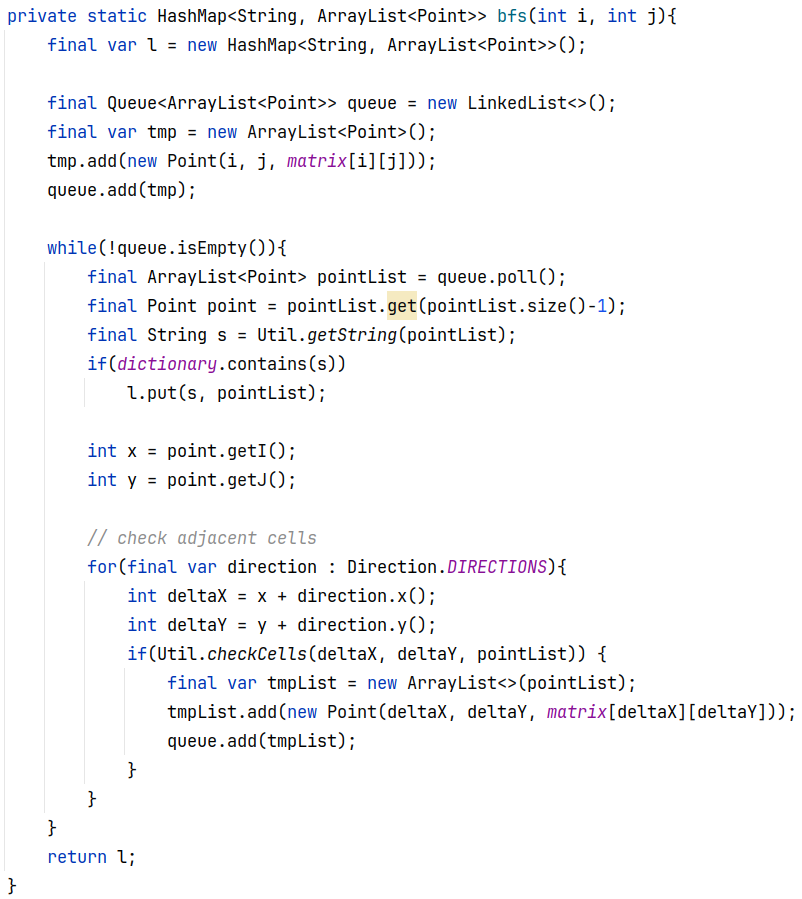
\includegraphics[width=1\textwidth]{bfs}
		Ricerca in ampiezza - implementazione in Java
		\newpage
	\end{center}
	\subsection{Ricerca in profondità}
	La ricerca in profondità fa la stessa cosa della ricerca in ampiezza, ma in modo diverso. Infatti, non espande i nodi come un pendolo ma procede analizzando \textbf{un ramo alla volta della matrice}. Dunque raggiunge immediatamente il livello più profondo della matrice, dove i nodi non hanno successori. L’espansione di tali nodi li rimuove dalla frontiera, per cui la ricerca “torna indietro” (backtracking) per riconsiderare il nodo più profondo che ha successori non ancora espansi. L'implementazione è molto simile a quello della ricerca in ampiezza, solo che la frontiera fa uso di una coda LIFO (Stack), poiché verrà sempre espanso l’ultimo nodo generato. Di questo tipo di ricerca ne esiste anche una versione ricorsiva, in cui lo Stack è implicitamente fornito dalle chiamate ricorsive.\\
	Questo algoritmo presenta dei \textbf{problemi} nel momento in cui l’albero di ricerca ha uno spazio degli stati con profondità infinita o con cicli, infatti l’algoritmo non terminerà. Quindi, possiamo sostenere che l’algoritmo di ricerca in profondità non è completo.
	Ma in questo caso, l'albero di ricerca è rappresentato da una matrice di cardinalità finita, che evita stati ripetuti e cammini ridondanti, quindi la ricerca è completa, se la soluzione esiste, perché alla fine espanderà tutti i nodi.\\
	Anche qui partiranno 16 ricerche in profondità, una per ogni casella.\\
	La complessità temporale resta uguale a quello della ricerca in ampiezza, ovvero O($b^m$) , dove m è la profondità massima di un nodo. Mentre lo spazio occupato è O(m), perché fa uso di backtracking, quindi non avremo mai uno Stack di taglia superiore a m. Da sottolineare che m può essere più grande di d.\\
	Questi algoritmi appena presentati risultano facili nella loro implementazione, ma poco interessanti sia per quanto riguarda la loro complessità asintotica, ma anche da un punto di vista di come viene risolto il problema, poiché alla fine tutto si riduce al bruteforce, ovvero provare tutte le combinazioni possibili. Già dal prossimo algoritmo vederemo qualcosa di più interessante.\\
	\small{\textit{Non verrà riportato il codice di questo algoritmo in quanto ritenuto simile a quello mostrato precedentemente.}}\\
	\subsection{Ricerca ad approfondimento iterativo}
	La ricerca ad approfondimento iterativo, oltre a migliorare la ricerca in profondità, è analoga a quella in ampiezza, poiché ad ogni iterazione esplora completamente un livello di nodi prima di prendere in considerazione il successivo. In altri termini, inizialmente l'algoritmo effettua le operazioni di ricerca nei nodi poco profondi, quelli vicini al nodo radice, \textbf{aumentando progressivamente la profondità} di scansione nei cicli di ricerca successivi. Tutto ciò migliorando i costi, senza compromettere la completezza.\\
	Nel nostro caso, facciamo partire una ricerca ad approfondimento iterativo per ogni vocabolo del dizionario, quindi partiranno 661.563 ricerche.
	\begin{lstlisting}
	foundWords = []
	for word in dictionary:
		wordIsFound = False
		for i=0; i < matrix.size &&  !wordIsFound; i++ :
			for j=0; j < matrix.size &&  !wordIsFound; j++ :
				result = approfondimentoIterativo(word, i, j)
				if result != NULL:
					foundWords += result
					wordIsFound = True
	\end{lstlisting}
	L'algoritmo di ricerca ad approfondimento iterativo come parametri prende in input: la parola da trovare e le coordinate (i,j) della casella da cui iniziare la ricerca. Quindi, come prima cosa verifica che il primo carattere della stringa passata sia uguale al contenuto della casella iniziale, se così non fosse l'algoritmo ritorna NULL.
	Dopo aver verificato questo step, l'algoritmo passa alla fase successiva, ovvero all'esplorazione dell'albero. In quanto richiede uno Stack per poter gestire la frontiera, può essere implementata in modo ricorsivo, come da noi fatto. Questa volta non vengono espansi tutti i nodi adiacenti allo stato attuale, ma solamente i nodi che contengono il carattere utile per la costruzione completa della stringa. Quindi ogni iterazione dell'esplorazione aggiunge un carattere alla stringa che stiamo trovando, l'esplorazione finisce quando troviamo la stringa completa (successo), oppure quando nessun nodo adiacente interessante (insuccesso).
	Analizzando la complessità, possiamo notare come nel caso pessimo saranno generati O($b^d$) nodi, mentre dovremo memorizzare solo un solo cammino dalla radice ad un nodo foglia, insieme ai rimanenti nodi fratelli non espansi per ciascun nodo sul cammino. Una volta che un nodo è stato espanso, può essere rimosso dalla memoria non appena tutti i suoi discendenti	sono stati esplorati completamente. Per cui, la complessità sarà di O(bd).
	\begin{center}
		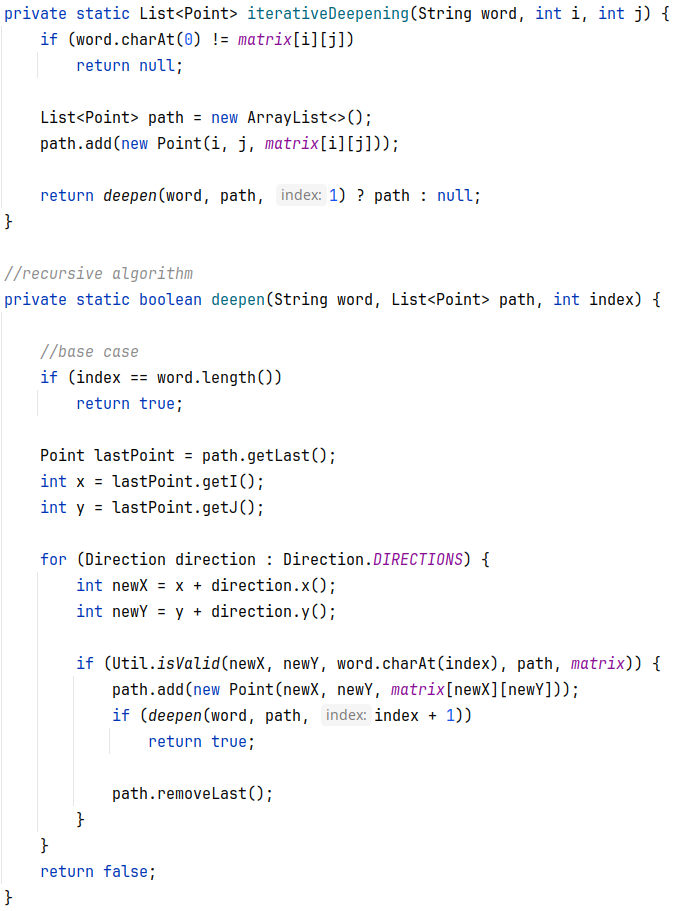
\includegraphics[width=1\textwidth]{iterativeDeepening}
		Ricerca ad approfondimento iterativo - implementazione in Java
		\newpage
	\end{center}
	\section{Ricerca informata}
	A questo punto, per migliorare i nostri algoritmi da un punto di vista computazionale, abbiamo deciso di implementare degli algoritmi di ricerca informata.
	Una strategia di ricerca informata può trovare soluzioni in modo più efficiente di una strategia non informata perché oltre a conoscere gli stati del problema conosce informazioni aggiuntive sul problema. Abbiamo pensato di dare più conoscenza all'algoritmo rappresentando il dizionario non più tramite un semplice Set di stringhe, ma con un'altra struttura dati, il Trie.\\\\
	\begin{large}
		\textbf{Trie}\\
	\end{large}
	Un Trie è una struttura dati ad albero utilizzata principalmente per memorizzare un set di stringhe, dove le chiavi sono generalmente sequenze di caratteri. La struttura del trie consente una \textbf{ricerca efficiente}, inserimento e cancellazione di stringhe. Ogni nodo dell'albero rappresenta un singolo carattere, mentre i percorsi dalla radice alle foglie rappresentano le stringhe. Quindi cercare una stringa all'interno di questa struttura costa $\Theta$(n), dove n è la lunghezza della stringa. La radice dell'albero è un carattere comune a tutte le stringhe, ovvero un carattere vuoto.\\
	Un trie è particolarmente utile in applicazioni che coinvolgono operazioni di prefissi, come nel nostro caso, infatti, data una stringa, possiamo cercare anche quali sono i caratteri successivi utili per formare una parola appartenente al dizionario. Questa funzionalità risulta utile durante l'esplorazione della matrice, infatti permette di poter escludere eventuali nodi che non portano alla costruzione di una parola di senso compiuto, evitando di esplorare stati inutili.
	L'idea di utilizzare questa struttura ci è venuta inspirandoci alla codifica di Huffman, studiata durante l'esame di \textit{Progettazione Algoritmi}, ma sopratutto abbiamo pensato a come noi esseri umani \textbf{sfogliamo un dizionario cartaceo}, infatti, partiamo sempre cercando il primo carattere della parola andando in ordine alfabetico, successivamente il secondo, poi il terzo...
	\begin{center}
		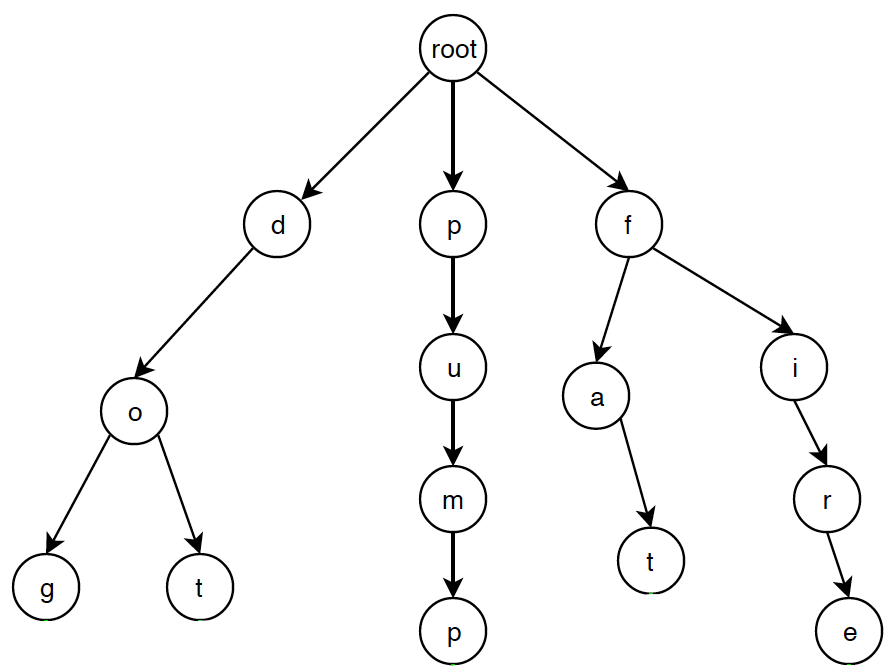
\includegraphics[width=1\textwidth]{trie}
		\small{Questo è un esempio di Trie dopo aver inserito i seguenti vocaboli: \textit{dog, dot, pump, fat, fire}.}
		\newpage
	\end{center}
	\subsection{Ricerca in ampiezza con Trie}
	Non c'è molta differenza con quanto già visto precedentemente nella ricerca in ampiezza, infatti l'esplorazione avviene allo stesso modo. La differenza sostanziale sta nel fatto che, nel corso della ricerca, \textbf{espandiamo solo i nodi i quali contengono caratteri potenziali per la costruzione di una parola del dizionario}.\\
	Cerchiamo di chiarirci con un esempio: arrivati ad un certo punto dell'esplorazione, estraggo dalla coda una lista di coordinate le quali formano la parola "ABAC". Passando codesta stringa al metodo \textit{searchBySubstring("ABAC")}, il Trie ci dirà che gli unici caratteri utili per formare una parola del dizionario sono: 'A', 'H', 'O' (le parole in questione sono: "ABACA", "ABACHI", "ABACHISTA", "ABACHISTE", "ABACHISTI", "ABACO").\\
	Quindi escluderemo dalla ricerca i nodi adiacenti che non contengono questi 3 caratteri.\\
	Quest'algoritmo mantiene le caratteristiche della ricerca in ampiezza classica, infatti esso è completo e la sua complessità sia temporale che spaziale è di O($b^d$); ma come abbiamo detto durante il corso, esiste esponenziale ed esponenziale.\\
	Anche perché in questa versione andiamo a diminuire il fattore di ramificazione b, infatti risulta difficile che un nodo possa visitare tutti e 8 i suoi nodi adiacenti, sopratutto negli step avanzati dell'algoritmo.\\
	Possiamo vedere da questi test come le prestazioni migliorino di molto se confrontate con la sua versione classica.
	\begin{center}
		\begin{tabular}{ |p{2cm}||p{3cm}|p{3cm}| }
			\hline
			& Parole trovate & Tempo impiegato\\
			\hline
			Senza Trie & 79 & 4.45196 s \\
			Con Trie & 79 & 0.00598925 s \\
			\hline
		\end{tabular}
	\end{center}
	La griglia data in input è la seguente:
	\begin{tabular}{ |c c c c| } 
		\hline
		A & B & C & D \\ 
		E & F & G & H \\ 
		I & L & M & N \\ 
		O & P & Q & R \\
		\hline
	\end{tabular}
	\begin{center}
		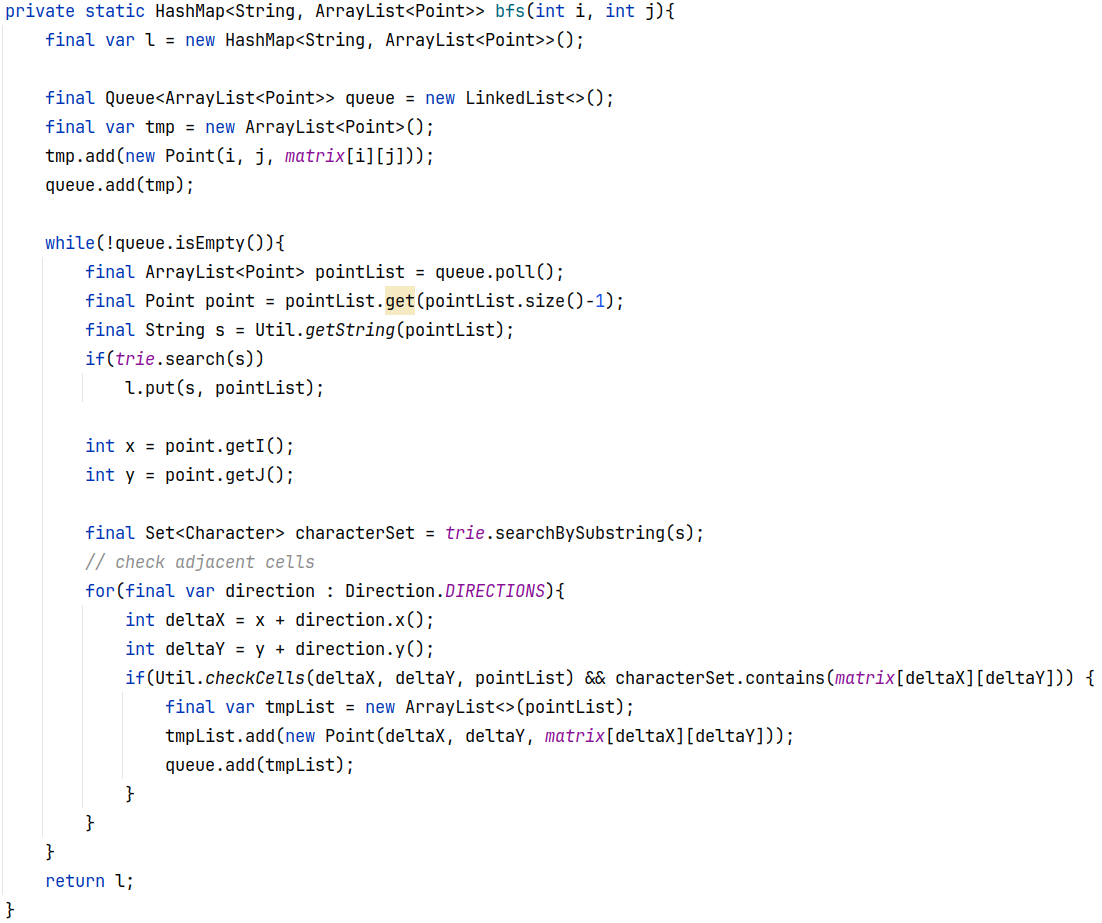
\includegraphics[scale=0.55]{bfsTrie}
		Ricerca in ampiezza con Trie - implementazione in Java
	\end{center}
	\subsection{Ricerca in profondità con Trie}
	Non vogliamo dilungarci troppo su quest'algoritmo in quanto esso è figlio della ricerca in profondità, quindi mantiene le sue caratteristiche già descritte. Alla ricerca vengono aggiunte le funzionalità del Trie, già descritte nel paragrafo precedente.
	\section{Considerazioni finali}
	Concludiamo dicendo che lavorare a questo progetto è stato utile per comprendere meglio le nozioni apprese durante il corso da un punto di vista pratico. Infatti, durante lo sviluppo, sono emerse altre interessanti idee di progetto, chissà, magari le svilupperemo in futuro..\\
	Con questa documentazione speriamo di aver fatto un buon lavoro, tanto da meritarci un posto tra le documentazioni presenti sulla piattaforma E-Learning, per ispirare le prossime generazioni di studenti.
\end{document}
